\documentclass[10pt]{beamer}
\usetheme[progressbar=frametitle]{metropolis}
\setbeamertemplate{frame numbering}[fraction]
\usecolortheme{beaver}
\usepackage{graphicx}
\usepackage{tikz}
\usepackage{listings} % for code
\usetikzlibrary{fadings}

\setbeameroption{show notes}
\setbeameroption{show notes on second screen=top}

\title{Linux Power!}
\subtitle{(From the perspective of a PMIC vendor)}
\author{Matti Vaittinen}
\institute{ROHM Semiconductors}
\date{Jan 10 2023}

\setbeamercovered{transparent=25}

\begin{document}

%-------------- title
\addtocounter{framenumber}{-1}


\begin{frame}[plain]
\note{Welcome. I am not excited to be here. I am terrified}
	\titlepage
\end{frame}

%-------------- topic page

\metroset{block=fill}

\begin{frame}[t]{Topics} \vspace{4pt}
\begin{block}{Goal}
What is PMIC \\
Regulator errors and notifications \\
Functional-safety helpers in regulator subsystem
\end{block} \vspace{8pt}

\tableofcontents
\note[item]{Shallow overview on what is PMIC and why it is needed}
\note[item]{Linux oriented Short glance of drivers can be needed for a PMIC}
\note[item]{functional safety and reporting hw issues}

\end{frame}

%-------------- about me page

\begin{frame}{About Me}
	\begin{columns}
	\column{0.58\linewidth}
		\begin{itemize}
			\item Matti Vaittinen
			\item Kernel/Driver developer at ROHM Semiconductor
			\item Worked at Nokia BTS projects (networking, clock \& sync) 2005 – 2017
			\item Currently mainly developing/maintaining upstream Linux device drivers for ROHM ICs
		\end{itemize}
	\column{0.38\linewidth}
		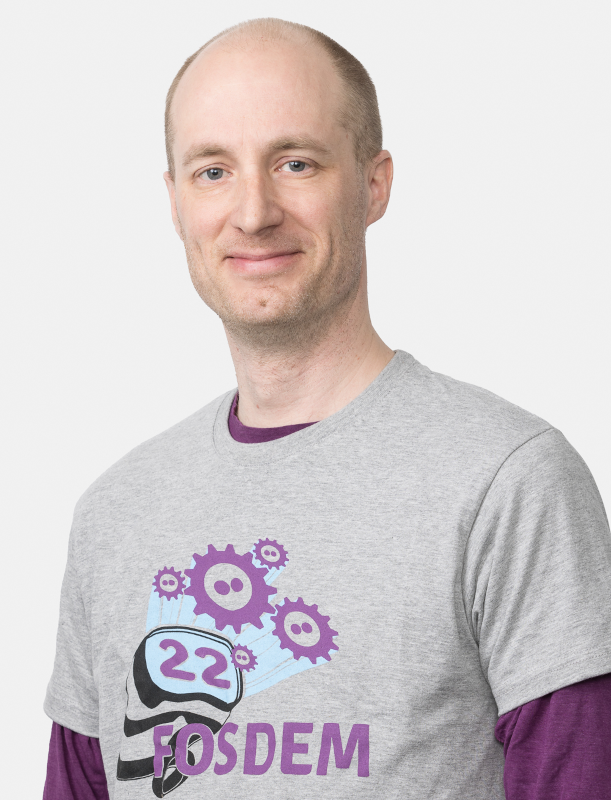
\includegraphics[width=1\linewidth]{img/me.png}
	\end{columns}
\note[item]{HW vendor, no forest from the trees.}
\note[item]{ Anyone with insight on how notifiers are or could be used - please explain!}
\end{frame}

%-------------- Powering a processor page

%Arrow style for all of the drawings
\tikzstyle{arrow} = [thick,->,>=stealth]

%Large SOC/PSY boxes
\tikzstyle{psys} = [rectangle, rounded corners, minimum width=3cm, minimum height=3cm,text centered, text width=3cm, draw=black, fill=red!30]
\tikzstyle{socs} = [rectangle, rounded corners, minimum width=3cm, minimum height=3cm,text centered, text width=3cm, draw=black, fill=green!30]

\addtocounter{framenumber}{-1}
\begin{frame}[plain]
\section{What and Why is a PMIC?}
\end{frame}

\begin{frame}[t]{Powering a processor}\vspace{4pt}
\begin{itemize}
	\item Processor and peripherals need power
	\item Can be as simple as a dummy DC power source with correct voltage
\end{itemize}


\vfill
\centering
\begin{minipage}[c]{.75\textwidth}
%  \flushright

\begin{tikzpicture}[node distance=5cm]
	\node (psy) [psys] {DC-source};
	\node (soc) [socs, right of=psy] {SOC};
	\draw [arrow] (psy) -- node[anchor=south] {+5V} (soc);
\end{tikzpicture}
\end{minipage}
\note{could be this simple. Just passive source}
\end{frame}

%-------------- Powering a modern SOC page

%Small PSY clk and SOC boxes
\tikzstyle{s_psys} = [rectangle, rounded corners, minimum width=2cm, minimum height=0.5cm,text centered, text width=2cm, draw=black, fill=red!30]
\tikzstyle{s_clk} = [rectangle, rounded corners, minimum width=2cm, minimum height=0.5cm,text centered, text width=2cm, draw=black, fill=orange!40]
\tikzstyle{s_socs} = [rectangle, rounded corners, minimum width=2.5cm, minimum height=3cm,text centered, text width=2.5cm, draw=black, fill=green!30]

\begin{frame}{Powering a modern SOC 1/2}
	\begin{columns}[onlytextwidth]
	\column{0.25\linewidth}

	 Modern SOCs can require multiple specific voltages

	\column{0.72\linewidth} \vspace{4pt}

	\begin{tikzpicture}[node distance=0.6cm]
		\node (nvcc_snvs) [s_psys] {LDO1 1.8V};
		\node (vdd_snvs) [s_psys, below of=nvcc_snvs] {LDO2 0.8V};
		\node (rtc_clk) [s_clk, below of=vdd_snvs] {RTC-CLK};
		\node (vdd_soc) [s_psys, below of=rtc_clk] {BUCK1 0.8V};
		\node (vdd_gpu) [s_psys, below of=vdd_soc] {BUCK5 0.9V};
		\node (vdd_phy) [s_psys, below of=vdd_gpu] {LDO4 0.9V};
		\node (vdd_arm) [s_psys, below of=vdd_phy] {BUCK2 0.9V};
		\node (imx8) [s_socs, right of=vdd_arm, xshift=5cm]{SOC};
		\node (vdda_dram) [s_psys, below of=vdd_arm] {LDO3 1.8V};
		\node (nvcc_1v8) [s_psys, below of=vdda_dram] {BUCK7 1.8V};
		\node (nvcc_dram) [s_psys, below of=nvcc_1v8] {BUCK8 1.1V};
		\node (nvcc_3v3) [s_psys, below of=nvcc_dram] {BUCK6 3.3V};
		\node (vdd_phy_1v2) [s_psys, below of=nvcc_3v3] {LDO6 1.2V};
		\node (ldo5) [s_psys, below of=vdd_phy_1v2] {LDO5 3.3V};

		\draw [arrow] (nvcc_snvs) node[anchor=south, xshift=3cm] {\scriptsize NVCC-SNVS} -|  ([xshift=1.6cm] imx8);
		\draw [arrow] (vdd_snvs) node[anchor=south, xshift=3cm] {\scriptsize VDD-SNVS} -| ([xshift=0.5cm] imx8);
		\draw [arrow] (rtc_clk) node[anchor=south, xshift=3cm] {\scriptsize RTC-CLK} -| ([xshift=-0.5cm] imx8);
		\draw [arrow] (vdd_soc) node[anchor=south, xshift=3cm] {\scriptsize VDD-SOC-VDDA-PHY} -| ([xshift=-1cm] imx8);
		\draw [arrow] (vdd_gpu) -- node[anchor=south]{\scriptsize VDD-GPU-VPU-VRAM} (imx8.west|-vdd_gpu) ;
		\draw [arrow] (vdd_phy) -- node[anchor=south] {\scriptsize VDD-PHY} (imx8.west|-vdd_phy);
		\draw [arrow] (vdd_arm) -- node[anchor=south] {\scriptsize VDD-ARM} (imx8.west|-vdd_arm);
		\draw [arrow] (vdda_dram) -- node[anchor=south] {\scriptsize VDDA-DRAM-VDDA} (imx8.west|-vdda_dram);
		\draw [arrow] (nvcc_1v8) -- node[anchor=south] {\scriptsize NVCC} (imx8.west|-nvcc_1v8);
		\draw [arrow] (nvcc_dram) node[anchor=north, xshift=3cm] {\scriptsize NVCC-DRAM} -| ([xshift=-1cm] imx8);
		\draw [arrow] (nvcc_3v3) node[anchor=north, xshift=3cm] {\scriptsize NVCC-3V3} -| ([xshift=-0.5cm] imx8);

		\draw [arrow] (vdd_phy_1v2) node[anchor=north, xshift=3cm] {\scriptsize VDD-PHY-1V2} -| ([xshift=0.5cm] imx8);
		\draw [arrow] (ldo5) node[anchor=north, xshift=3cm] {\scriptsize LDO5-OUT} -| ([xshift=1.6cm] imx8);
	\end{tikzpicture}
	\end{columns}
\note[item]{almost a real SOC.}
\note[item]{pic omits state GPIOs}
\end{frame}

%-------------- Powering a modern SOC page 2

\begin{frame}{Powering a modern SOC 2/2}
	\begin{columns}[onlytextwidth]
	\column{0.18\linewidth}
		And specific timings...
	\column{0.82\linewidth}\vspace{4pt}
		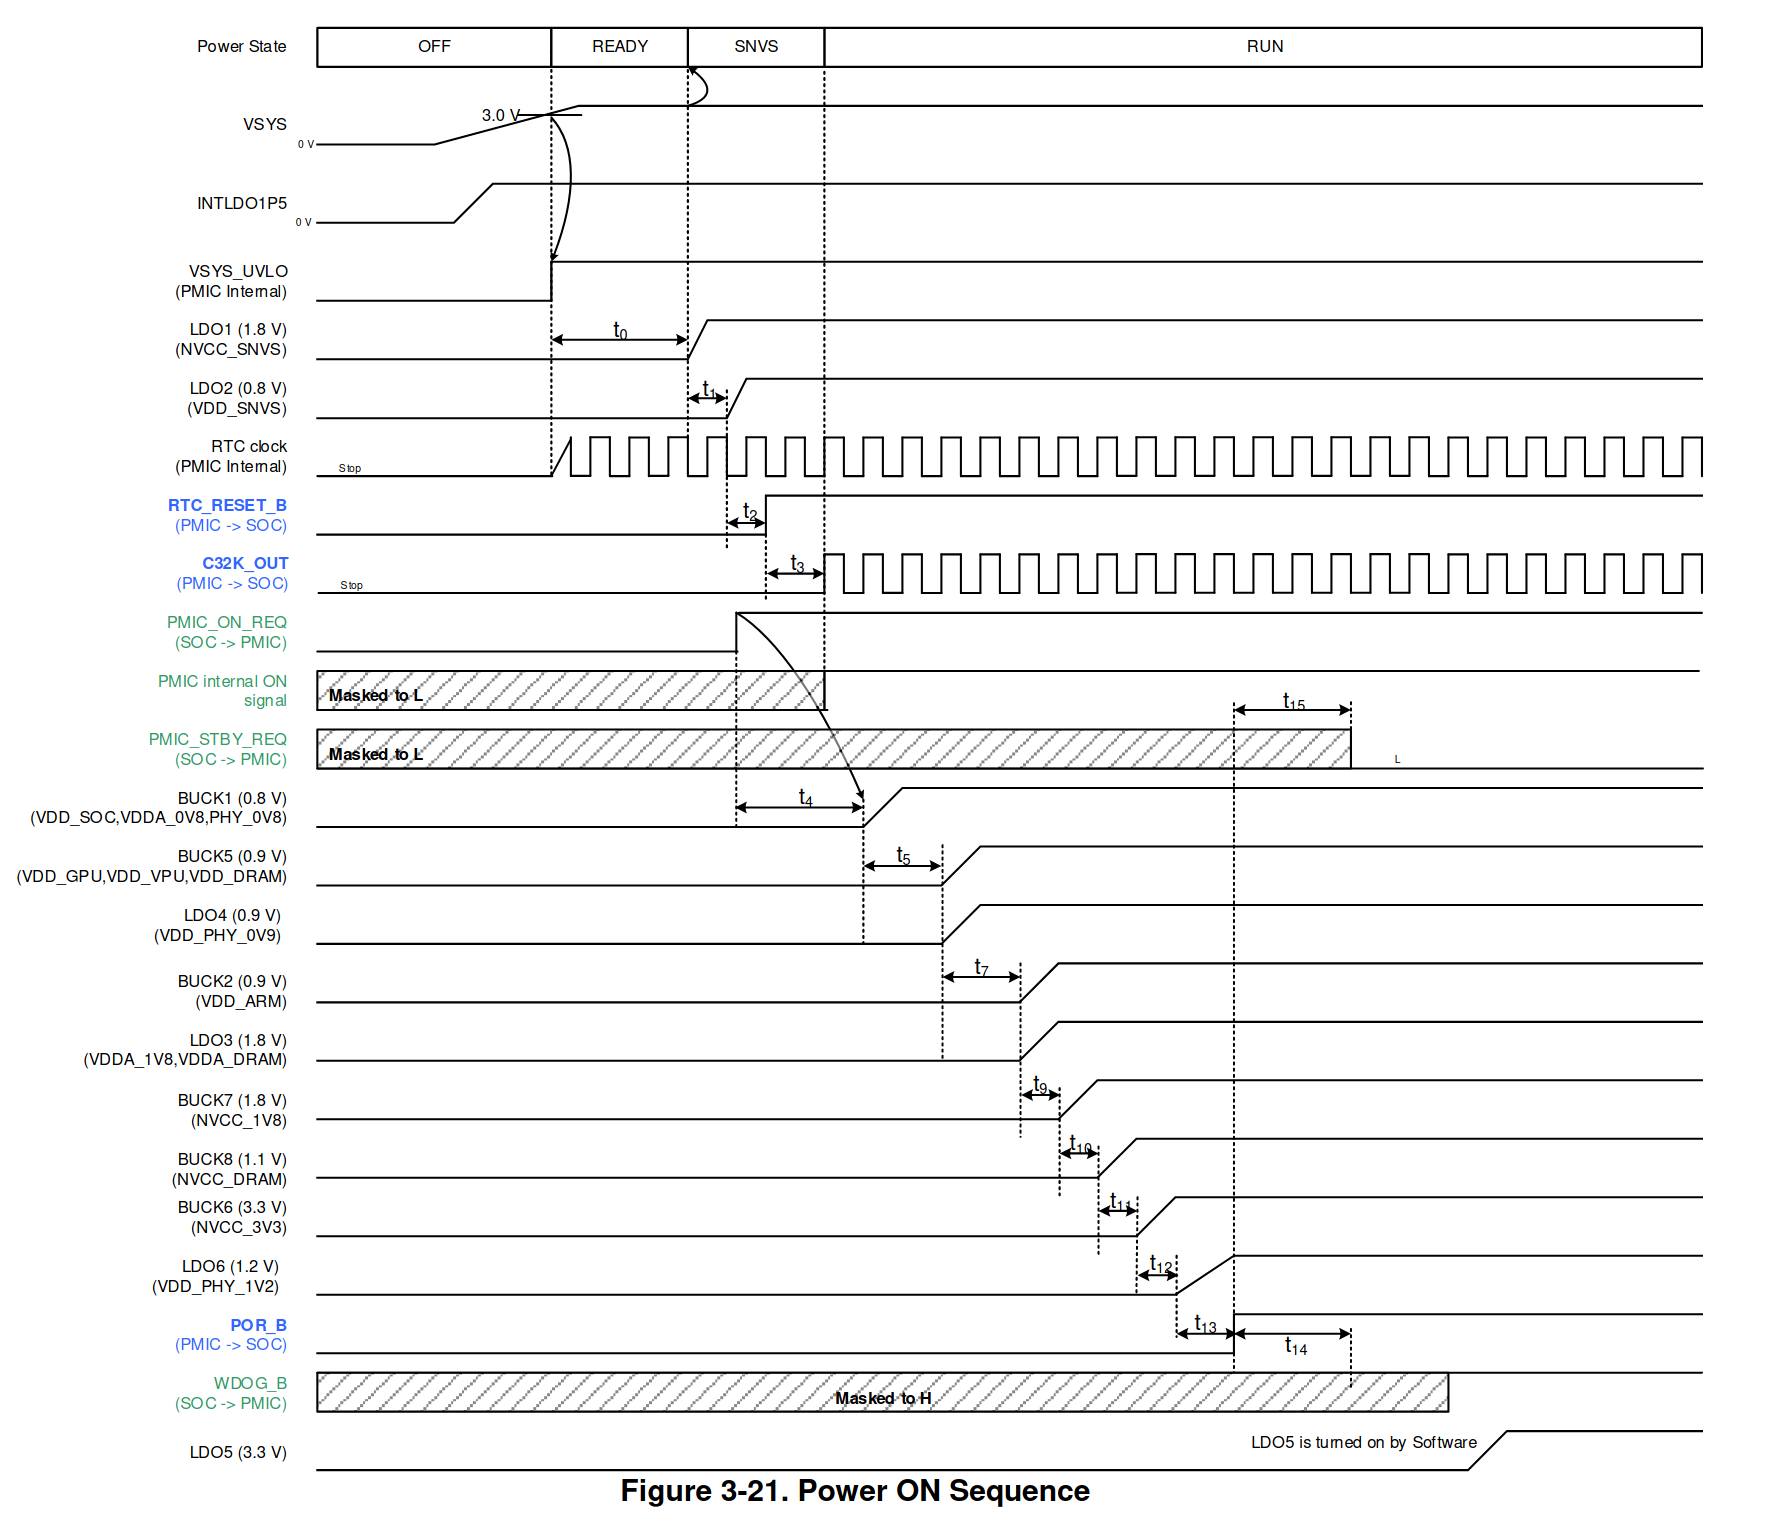
\includegraphics[width=1\linewidth]{img/BD71847_start_up_seq.png}
	\end{columns}
\note[item]{TIMINGs - explain state transitions}
\note[item]{from PMIC spec}
\note[item]{shows also internal changes}
\end{frame}

%-------------- More control page

\begin{frame}{More control...}
Power savings by:
\begin{itemize}
	\item Shutting down not needed devices
	\item Stand-by state(s)
	\item DVS (Dynamic Voltage Scaling)
\end{itemize}
\note[item]{Importance of power saving increases}
\note[item]{Toggling outputs on/off}
\note[item]{Changing voltages}
\note[item]{Predefined states changed by GPIO (avoid I2C shut-down races I2C depends on some other block - other can't be shut down?)}
\end{frame}

%--------------  Automated power-on page

\begin{frame}{Automated power on}
Powering-on a system at given time...
\begin{itemize}
	\item RTC
\end{itemize}
...Or by an event
\begin{itemize}
	\item HALL sensor, ...
\end{itemize}
\note[item]{Monitor turn-on  input when SOC is shut down}
\note[item]{For example RTC / HALL sensor (lid) }
\end{frame}

%--------------  More requirements page

\begin{frame}{More requirements...}
\begin{itemize}
	\item Battery / charger
	\item Watchdog
	\item Functional-safety
	\begin{itemize}
		\item Voltage monitoring
		\item Current monitoring
		\item Temperature monitoring
	\end{itemize}
\end{itemize}
\note{More needs}
\note[item]{battery powered devices everywhere => charging logic}
\note[item]{Watchdog cut power - can be external or in power-supply}
\note[item]{montor abnormal events (temp, over voltage, ocp)}
\end{frame}

%--------------  PMICs page

\newcommand\TBox[2][]{%
  \tikz\node[draw,minimum width=1.8cm,minimum height=1cm,text centered,rounded corners,ultra thick,align=center,#1] {#2};}

\begin{frame}{PMICs}
PMIC - Power Management Integrated Circuit
\begin{itemize}
	\item Multiple DC sources with specific start-up / shut-down sequence
	\item Voltage control
	\item Functional-safety
	\item Auxiliary blocks to support various needs\\ [10pt]
\end{itemize}

\TBox[fill=gray!30]{%
	\TBox[fill=red!30]{Regulators/Monitoring} PMIC \TBox[fill=cyan!30]{Battery/Charger} \\ 
	\TBox[fill=green!30]{Watchdog}\TBox[fill=green!30]{RTC}\TBox[fill=green!30]{CLK}\TBox[fill=green!30]{GPIO}} \\

%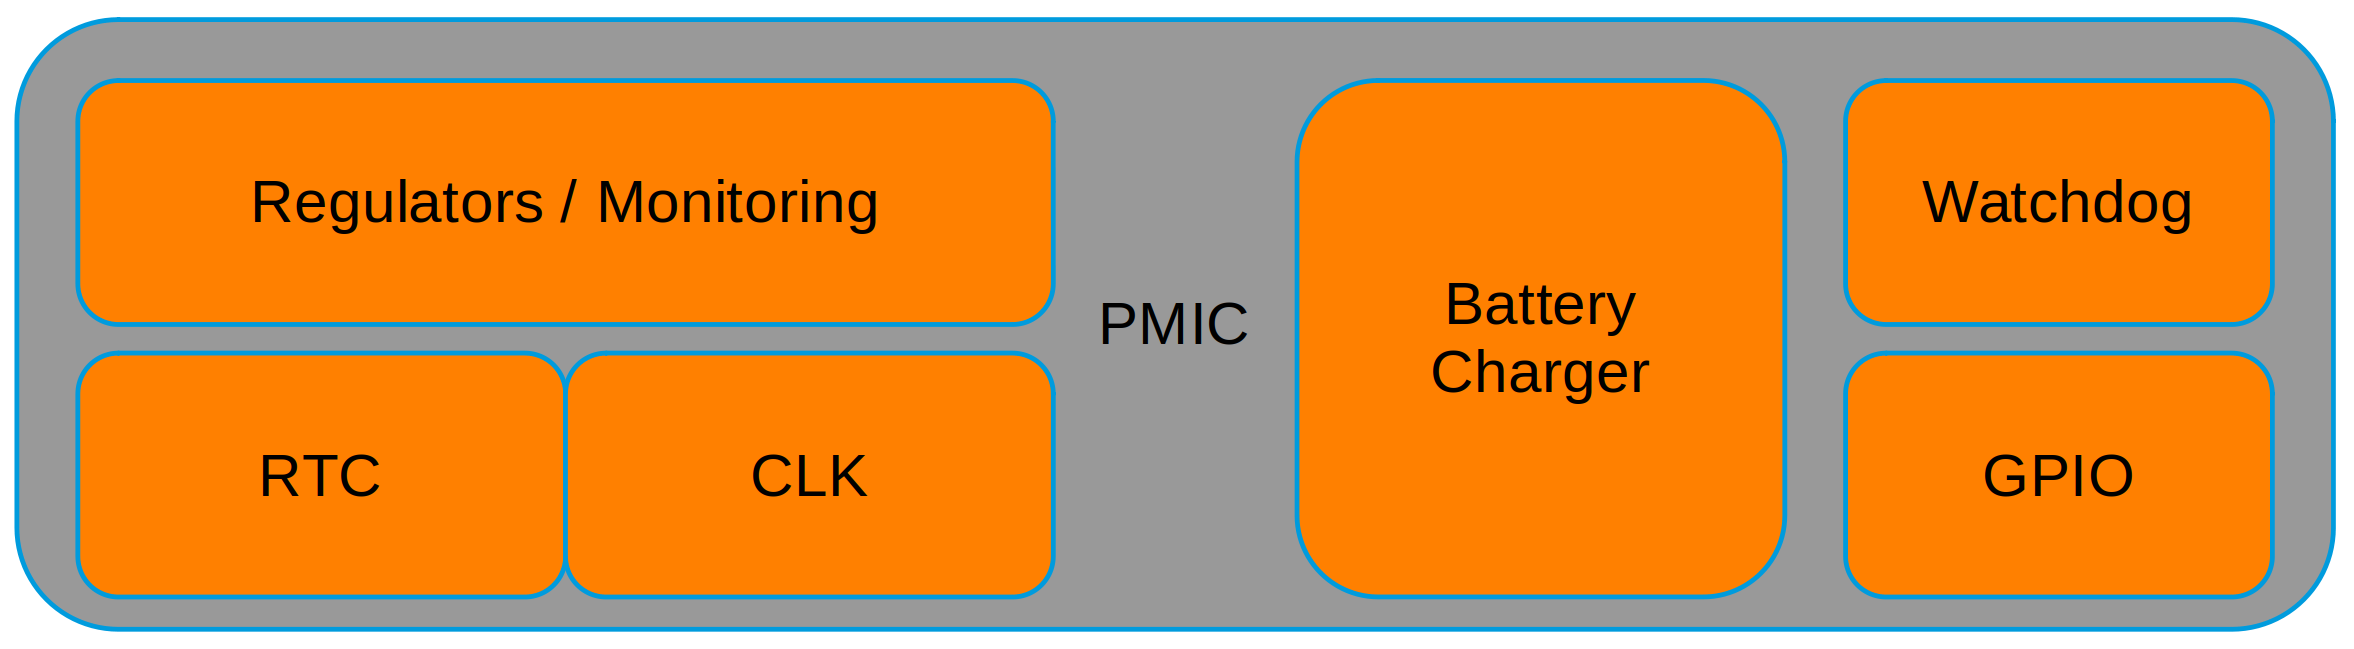
\includegraphics[width=1\linewidth]{img/pmic_block.png}
\end{frame}

%============== Section PMIC drivers

\addtocounter{framenumber}{-1}
\begin{frame}[plain]
\section{PMIC drivers}
\subsection{MFD and subdevices}
\subsection{Regulators}
\end{frame}

%--------------  MFD page

\begin{frame}[t]{Multi Function Devices}
	\begin{columns}
	\column[t]{0.3\linewidth}
\begin{block}{Often MFD drivers}
	\begin{itemize}
		\item \textbf{Regulator}
		\item RTC
		\item Power supply
		\item Watchdog
		\item GPIO
		\item CLK ...
	\end{itemize}
\end{block}
	\column[t]{0.68\linewidth}
		\only<1> {\textbf{Why?} (I have 1 reason on mind, may be more)}
		\only<2>{
			\textbf{Allows re-use \\[10pt]}
			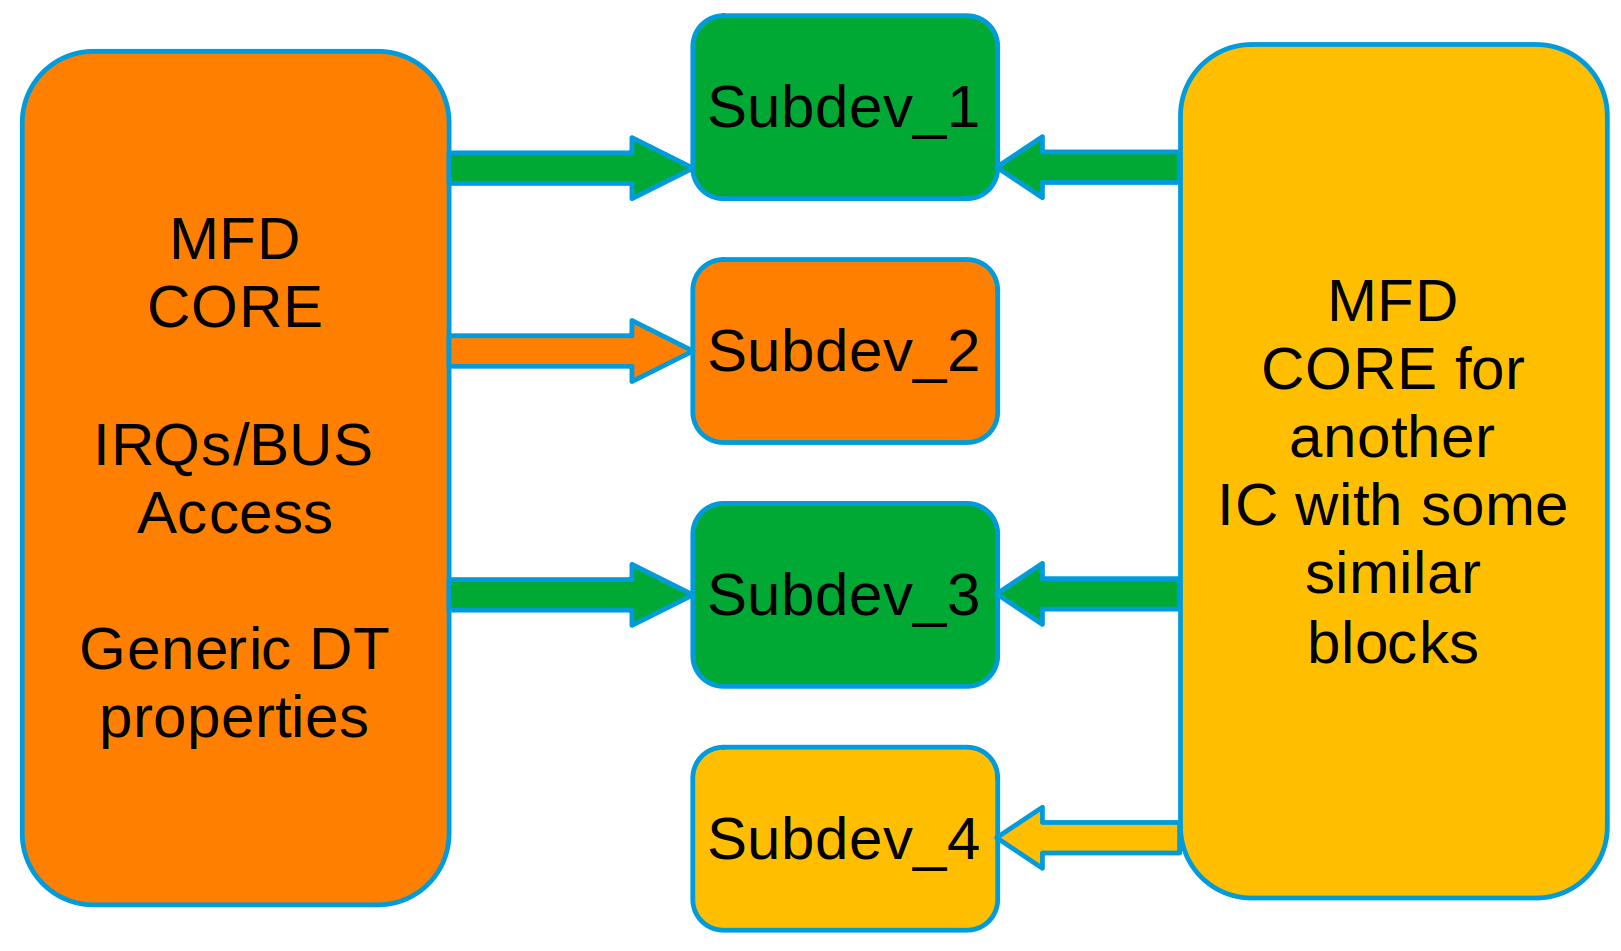
\includegraphics[width=1\linewidth]{img/MFD_re_use.png}
		}
	\end{columns}
\end{frame}

%--------------  regulator consumer/provider page

\begin{frame}[t]{Regulator (provider) and consumer}\vspace{4pt}
\begin{itemize}
	\item Provider is driver interfacing the hardware. Eg, sits “below” the regulator framework. Between regulator framework and HW
	\item Consumer is driver who wishes to control the regulator using the regulator framework. Eg, sits “on top of” the regulator framework
	\item PMIC driver is the provider driver (usually just referred as a regulator driver) \\[10pt]
\end{itemize}
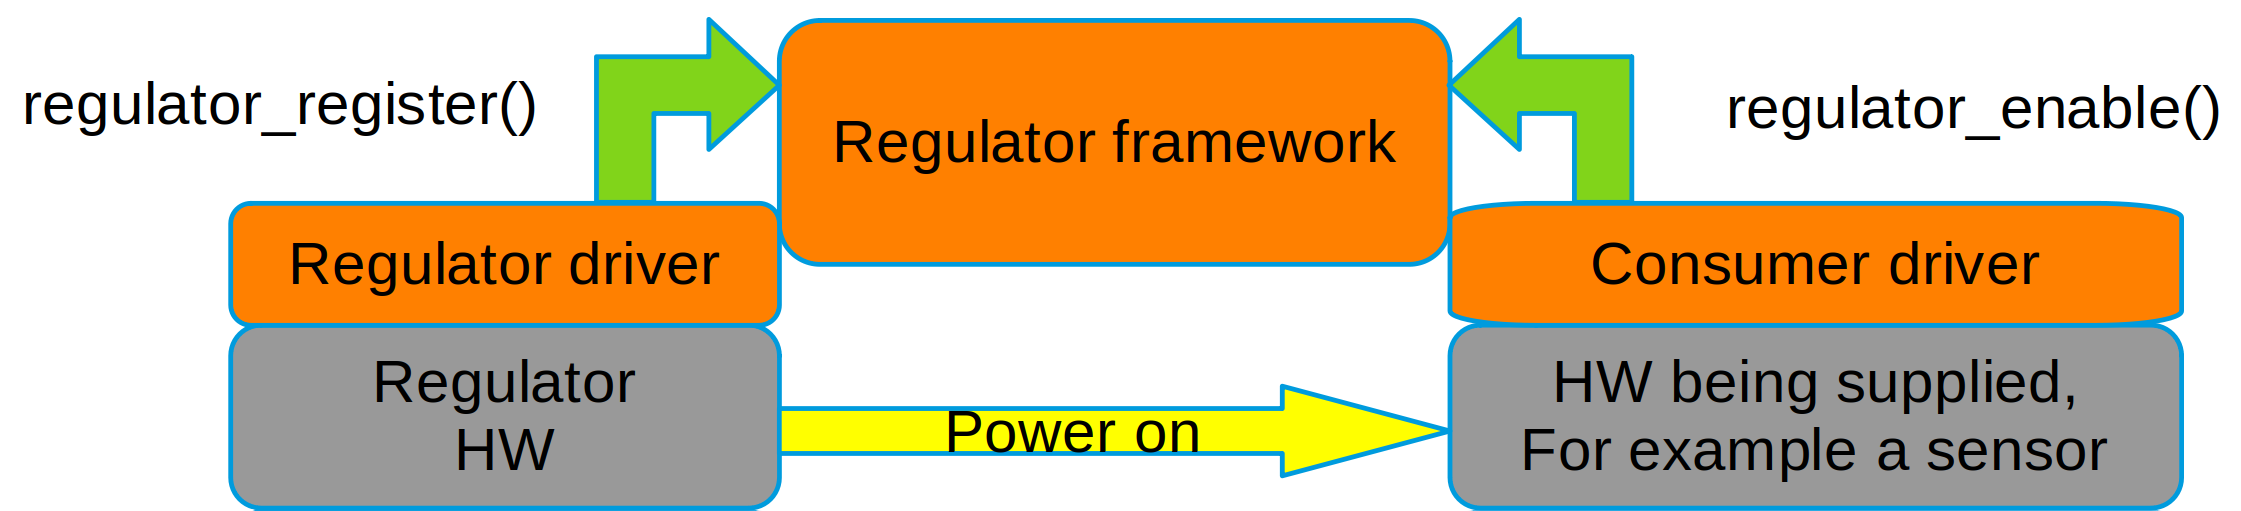
\includegraphics[width=1\linewidth]{img/regulator_users.png}
\end{frame}

%============== Section Functional-safety

\addtocounter{framenumber}{-1}
\begin{frame}[plain]
\section{Monitoring for abnormal conditions}
\subsection{Severity levels and limit values}
\subsection{Regulator errors and notifications}
\subsection{Helpers and examples}
\end{frame}


%-------------- notification / error flags page

\begin{frame}[t]{Detecting undexpected}\vspace{4pt}
\begin{block}{Linux has 3 severity categories}

\end{block}

\begin{itemize}
	\item  \textbf{PROTECTION}
\onslide<2>{
	\begin{itemize}
		\item Unconditional \textcolor{magenta}{shutdown by HW}
	\end{itemize}
}
	\item \textbf{ERROR}
\onslide<3>{
	\begin{itemize}
		\item \textcolor{red}{Irrecoverable error,} system not expected to be usable. Error handling by software.
	\end{itemize}
}
	\item  \textbf{WARNING} - NEW(ish)
\onslide<4>{
	\begin{itemize}
		\item \textcolor{orange}{Something is off-limit,} system still usable but a recovery action should be taken to prevent escalation to errors
	\end{itemize}
}
\end{itemize}
\end{frame}

%--------------  setting safety limits via device-tree page

\begin{frame}[t]{Safety limits, devicetree}\vspace{4pt}
\onslide<1-2>{
\begin{block}{Property format:}
\begin{itemize}
	\item  regulator-\textless event \textgreater-\textless severity \textgreater-\textless unit \textgreater = value
\end{itemize}
\end{block}

Over current:
\begin{itemize}
	\item regulator-oc-protection-microamp
	\item regulator-oc-error-microamp
	\item regulator-oc-warn-microamp
\end{itemize}

Similar for over voltage (oc), under voltage (uv) and temperature (temp)
}
\onslide<2>{
\par
Values:
\begin{itemize}
	\item 0 =\textgreater disable
	\item 1 =\textgreater enable
	\item other =\textgreater new limit
\end{itemize}
}

\only<3->{
\textcolor{red}{\textbf{What if hardware does not support given limit?}}
}
\end{frame}

%--------------  limit config callbacks page

\begin{frame}[fragile]{Callbacks for configuring the limits}
\lstset{language=C}
\scriptsize

\begin{lstlisting}
struct regulator_ops {
	// snip
	int (*set_over_current_protection)(struct regulator_dev *,
	       int lim_uA, int severity, bool enable);
	int (*set_over_voltage_protection)(struct regulator_dev *,
	      int lim_uV, int severity, bool enable);
	int (*set_under_voltage_protection)(struct regulator_dev *,
	     int lim_uV, int severity, bool enable);
	int (*set_thermal_protection)(struct regulator_dev *, int lim,
	     int severity, bool enable);
};
\end{lstlisting}
\pause

\begin{lstlisting}
struct regulator_desc {
	// snip
	const struct regulator_ops *ops;
};
 \end{lstlisting}
\pause

\begin{lstlisting}
struct regulator_dev *devm_regulator_register(struct device *dev,
			  const struct regulator_desc *regulator_desc,
			  const struct regulator_config *config);
\end{lstlisting}

\end{frame}

%--------------  page limiting Example


\begin{frame}[fragile]{Simplified example}
\lstset{language=C}
\scriptsize
\begin{lstlisting}[commentstyle=\color{orange}]
static int bd9576_set_ocp(struct regulator_dev *rdev, int lim_uA,
			  int severity, bool enable)
{
	...

	/* Return -EINVAL for unsupported configurations */
	if ((lim_uA && !enable) || (!lim_uA && enable))
		return -EINVAL;

	/*
	 * Select the correct register and appropriate register-value
	 * conversion for given severity and limit..
	 */
	if (severity == REGULATOR_SEVERITY_PROT) {
		...
	} else {
		...
	}

	/* Write configuration to registers */
	return bd9576_set_limit(range, num_ranges, d->regmap,
				reg, mask, Vfet);
}
\end{lstlisting}
\end{frame}

%--------------  informing the unexpected page

\begin{frame}[t]{Informing the unexpected}\vspace{4pt}
\begin{block}{Two types of information}
\begin{itemize}
	\item ERRORs
	\item NOTIFICATIONs
\end{itemize}
\end{block}

\begin{itemize}
\onslide<2->{
	\item  \textbf{ERROR}
	\begin{itemize}
		\item set by provider
		\item queried (polled) by consumer
		\item regulator$\_$get$\_$error$\_$flags()
	\end{itemize}
}
\onslide<3>{
	\item \textbf{NOTIFICATION}
	\begin{itemize}
		\item sent by provider (usually) from interrupt
		\item no polling needed
		\item regulator$\_$register$\_$notifier()
		\item can send also other events
	\end{itemize}
}
\end{itemize}
\end{frame}

%--------------  list of errors page

\begin{frame}[fragile]{Regulator error flags}
\begin{lstlisting}
#define REGULATOR_ERROR_UNDER_VOLTAGE
#define REGULATOR_ERROR_OVER_CURRENT
#define REGULATOR_ERROR_REGULATION_OUT
#define REGULATOR_ERROR_FAIL
#define REGULATOR_ERROR_OVER_TEMP
#define REGULATOR_ERROR_UNDER_VOLTAGE_WARN
#define REGULATOR_ERROR_OVER_CURRENT_WARN
#define REGULATOR_ERROR_OVER_VOLTAGE_WARN
#define REGULATOR_ERROR_OVER_TEMP_WARN
\end{lstlisting}
include/linux/regulator/consumer.h
\end{frame}

%--------------  list of notifications page

\begin{frame}[fragile]{Regulator notifications}
\begin{lstlisting}
#define REGULATOR_EVENT_UNDER_VOLTAGE
#define REGULATOR_EVENT_OVER_CURRENT
#define REGULATOR_EVENT_REGULATION_OUT
#define REGULATOR_EVENT_FAIL
#define REGULATOR_EVENT_OVER_TEMP
...
#define REGULATOR_EVENT_UNDER_VOLTAGE_WARN
#define REGULATOR_EVENT_OVER_CURRENT_WARN
#define REGULATOR_EVENT_OVER_VOLTAGE_WARN
#define REGULATOR_EVENT_OVER_TEMP_WARN
#define REGULATOR_EVENT_WARN_MASK
\end{lstlisting}
include/linux/regulator/consumer.h
\end{frame}

%--------------  Notifications page

\begin{frame}{Notifications}
Usually IRQ backed
\begin{enumerate}
	\item PMIC detects error and generates IRQ
	\item IRQ handler sends notification
	\item Regulator consumer action is executed
\end{enumerate}
\pause
In some (many) cases IRQ is held active for whole duration of error
\begin{itemize}
	\item Maybe because these IRQs are considered as a last thing?
	\item Maybe because there is need to ensure IRQ is not missed?
	\item Does not play well with all systems
\end{itemize}
\end{frame}

%-------------- IRQ helper page

\begin{frame}[fragile, t]{Event IRQ helper}\vspace{4pt}
\begin{block}{A helper provided for IRQ handling and sending the notification}
\begin{itemize}
	\item Supports keeping IRQ disabled for a period of time
	\item Supports forcibly shutting down the system if accesing the PMIC fails
\end{itemize}
\end{block}
\vfill
\lstset{language=C}
\scriptsize
\begin{lstlisting}
void *regulator_irq_helper(struct device *dev,
		   const struct regulator_irq_desc *d, int irq,
		   int irq_flags, int common_errs, 
		   int *per_rdev_errs, struct regulator_dev **rdev,
		   int rdev_amount);
\end{lstlisting}
\end{frame}

%-------------- Helper break-out page

\begin{frame}[t]{Helper break-out}\vspace{4pt}
\begin{columns}[onlytextwidth]
	\column[t]{0.25\linewidth}
	events
	\only<2->{
		
\includegraphics[width=1\linewidth]{img/isr/IRQ.png}
	}
	\only<4->{
		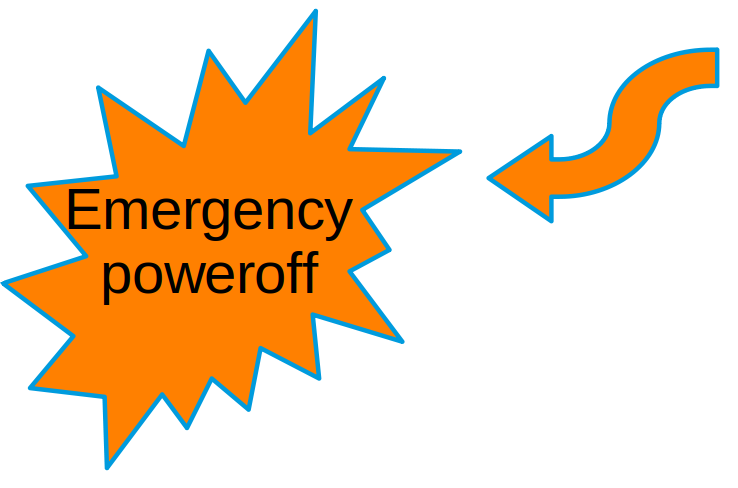
\includegraphics[width=1\linewidth]{img/isr/emergpoff.png}
	}
	\only<5->{
		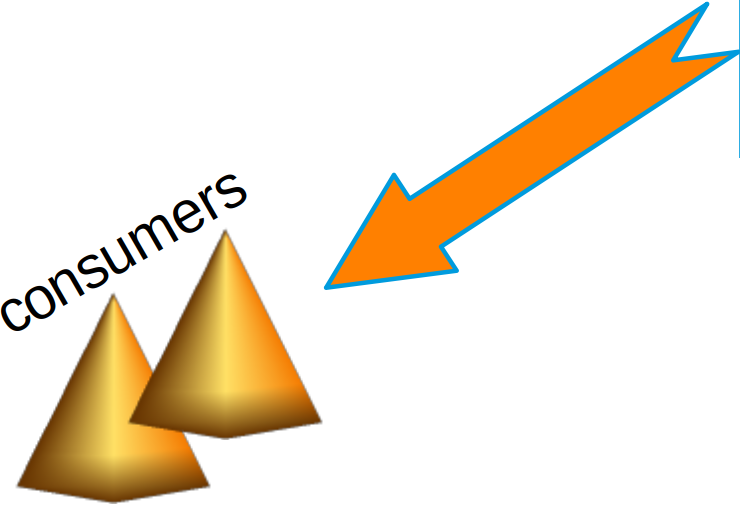
\includegraphics[width=1\linewidth]{img/isr/consumers.png}
	}
	\column[t]{0.25\linewidth}
	helper \\[4pt]
	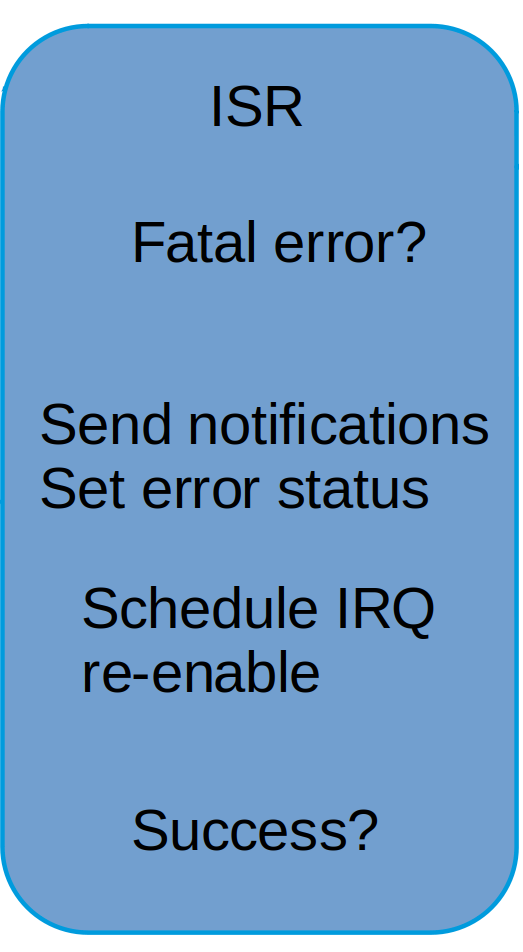
\includegraphics[width=1\linewidth]{img/isr/helperbox_size.png}
	\column[t]{0.20\linewidth}
	action \\[12pt]
	\only<3->{
		
\includegraphics[width=1\linewidth]{img/isr/map_event.png}
	}
	\only<4->{
		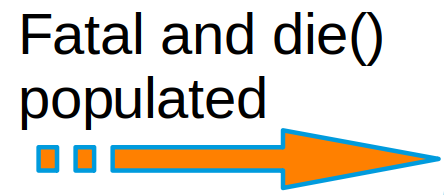
\includegraphics[width=1\linewidth]{img/isr/die.png}\vspace{20pt}
	}
	\only<6->{
		
\includegraphics[width=1\linewidth]{img/isr/renable.png}
	}
	\only<7->{
		
\includegraphics[width=0.5\linewidth]{img/isr/retry.png}
	}
	\column[t]{0.30\linewidth}
	driver \\[4pt]
	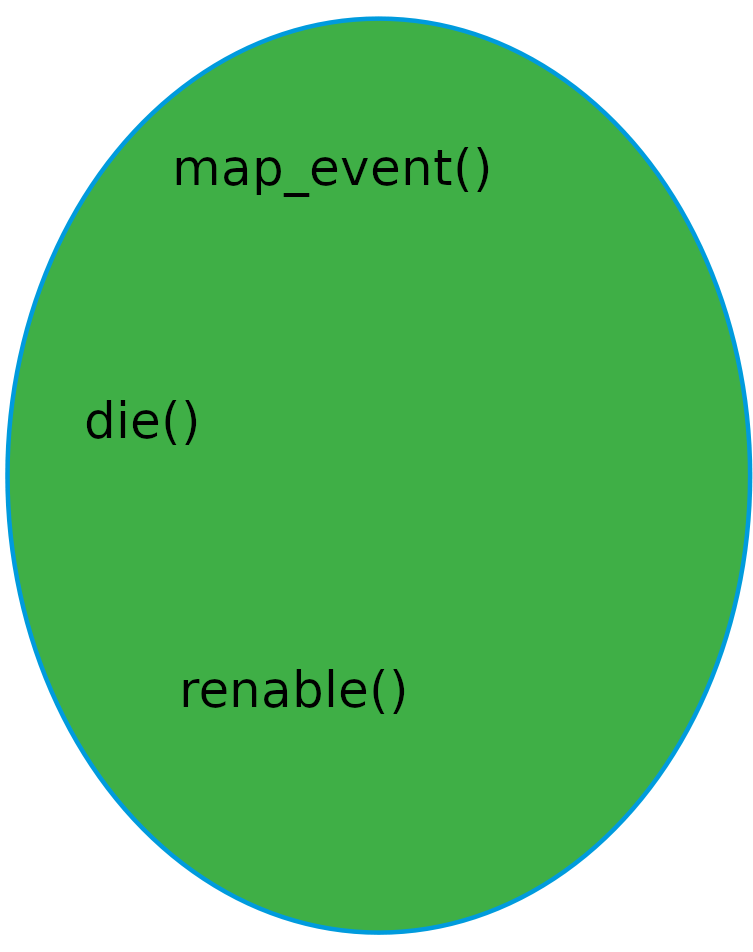
\includegraphics[width=1\linewidth]{img/isr/driver_size.png}
	\end{columns}
\end{frame}


%--------------  limit config callbacks page

\begin{frame}[fragile]{Helper configuration}
\lstset{language=C}
\scriptsize

\begin{lstlisting}
struct regulator_irq_desc {
	const char *name;
	int fatal_cnt;
 \end{lstlisting}
\pause
\begin{lstlisting}
	int reread_ms;
	int irq_off_ms;
 \end{lstlisting}
\pause
\begin{lstlisting}
	bool skip_off;
	bool high_prio;
 \end{lstlisting}
\pause
\begin{lstlisting}
	void *data;
	int (*die)(struct regulator_irq_data *rid);
	int (*map_event)(int irq, struct regulator_irq_data *rid,
	     unsigned long *dev_mask);
	int (*renable)(struct regulator_irq_data *rid);
};
 \end{lstlisting}
\pause

\begin{lstlisting}
void *regulator_irq_helper(struct device *dev,
		   const struct regulator_irq_desc *d, int irq,
		   int irq_flags, int common_errs, 
		   int *per_rdev_errs, struct regulator_dev **rdev,
		   int rdev_amount);
\end{lstlisting}
(or a devm-variant)
\end{frame}

%--------------  Event mapping page

\begin{frame}[fragile]{Event mapping}
\lstset{language=C}
\scriptsize

\begin{lstlisting}
int (*map_event)(int irq, struct regulator_irq_data *rid,
		 unsigned long *dev_mask);
 \end{lstlisting}
\pause
\begin{lstlisting}
struct regulator_irq_data {
	struct regulator_err_state *states;
	int num_states;
	void *data;
	long opaque;
};
 \end{lstlisting}
\pause
\begin{lstlisting}
struct regulator_err_state {
	struct regulator_dev *rdev;
	unsigned long notifs;
	unsigned long errors;
	int possible_errs;
};
 \end{lstlisting}
\pause

\begin{lstlisting}
int (*renable)(struct regulator_irq_data *rid);
 \end{lstlisting}
\pause

\begin{lstlisting}
int regulator_irq_map_event_simple(int irq,
			struct regulator_irq_data *rid,
			unsigned long *dev_mask)
 \end{lstlisting}
\end{frame}

%--------------  Event mapping example

\begin{frame}[fragile]{Event mapping example}
\lstset{language=C}
\scriptsize

\begin{lstlisting}
static int bd9576_ovd_handler(int irq, struct regulator_irq_data *rid,
			      unsigned long *dev_mask)
{
	ret = regmap_read(d->regmap, BD957X_REG_INT_OVD_STAT, &val);
	if (ret)
		return REGULATOR_FAILED_RETRY;

\end{lstlisting}

\pause
\begin{lstlisting}
	rid->opaque = val & OVD_IRQ_VALID_MASK;
	*dev_mask = 0;

	if (!(val & OVD_IRQ_VALID_MASK))
		return 0;
\end{lstlisting}
\pause
\begin{lstlisting}
	*dev_mask = val & BD9576_xVD_IRQ_MASK_VOUT1TO4;

	for_each_set_bit(i, dev_mask, 4) {
		stat  = &rid->states[i];

		stat->notifs	= rdata->ovd_notif;
		stat->errors	= rdata->ovd_err;
	}

	return 0;
}

\end{lstlisting}
\end{frame}


%--------------  Helper regisration example

\begin{frame}[fragile]{Helper registration 1/2}
\lstset{language=C}
\scriptsize

Fill the helper configuration
\pause
\begin{lstlisting}
static const struct regulator_irq_desc bd9576_notif_ovd = {              
       .name = "bd9576-ovd",                                            
       .irq_off_ms = 1000,                                              
       .map_event = bd9576_ovd_handler,                                 
       .renable = bd9576_ovd_renable,                                   
       .data = &bd957x_regulators,                                      
}; 
\end{lstlisting}
\end{frame}

\begin{frame}[fragile]{Helper registration 2/2}
\lstset{language=C}
\scriptsize

Create an array of regulators this IRQ may concern
\pause
\begin{lstlisting}
struct regulator_dev *rdevs[BD9576_NUM_REGULATORS];

for (i = 0; i < num_rdev; i++) {
	struct bd957x_regulator_data *r = &ic_data->regulator_data[i];
	const struct regulator_desc *desc = &r->desc;

	r->rdev = devm_regulator_register(&pdev->dev, desc, &config);

	rdevs[i] = r->rdev;
	if (i < BD957X_VOUTS1)
		ovd_devs[i] = r->rdev;
}
\end{lstlisting}
\pause
Fill possible errors this IRQ may indicate and register the helper
\pause
\begin{lstlisting}
int ovd_errs = REGULATOR_ERROR_OVER_VOLTAGE_WARN |
	 REGULATOR_ERROR_REGULATION_OUT;

ret = devm_regulator_irq_helper(&pdev->dev, &bd9576_notif_ovd,
				irq, 0, ovd_errs, NULL,
				&ovd_devs[0],
				BD9576_NUM_OVD_REGULATORS);

\end{lstlisting}
\end{frame}

%============== Section Wrap-up

\addtocounter{framenumber}{-1}
\begin{frame}[plain]
\section{Wrap it up}
\end{frame}

\begin{frame}{Summary}
\begin{itemize}
	\item Powering up a modern SOC is not simple
	\item PMIC is an IC trying to integrate powering related features into single chip
	\item Many PMICs include functional-safety features
	\item There is some existing support for indicating abnormal events
\end{itemize}
\end{frame}

\begin{frame}{No answers guaranteed}
\center
\only<1>{ \huge Questions?}
\only<2>{ \huge Thank You for listening! \\
(or time to wake up) :)}
\end{frame}

\end{document}
